\section{Verification}
Testing is important in software development to ensure that written code new and refactored are both fucntional and stable.
In this project there have been a focus on unit tests for important logic and Behavior-Driven Development (BDD) for user testing.

by doing unit testing and BDD together, it can ensure that both the functionality of the individual components and the overall user experience are done as
intended by the developers with the end user in mind.
by doing unit testing and BDD, it will help immensely with the software not only works as intended from a technical view point,
but also meets end users expectations in a given scenario.

\subsection{Unit Testing}

\subsubsection{JDisclosureToolBar Tests}
Unit tests for the \textit{JDisclosureToolBar} class are made to ensure its will be fucntional readable as intended.
For the JDisclosureToolBar class, unit tests were developed to check its key functionalities to make sure its working as inteded.
The focus for this unit tests was on the toolbars ability to update and retrieve state information correctly.


\subsubsection{testSetDisclosureStateCount}
This test is used to verify that the setDisclosureStateCount method updates the state count of the disclosure button correctly.
The test involves setting a new state count and confirming that the change is done correctly.

\begin{figure}[H]
    \centering
    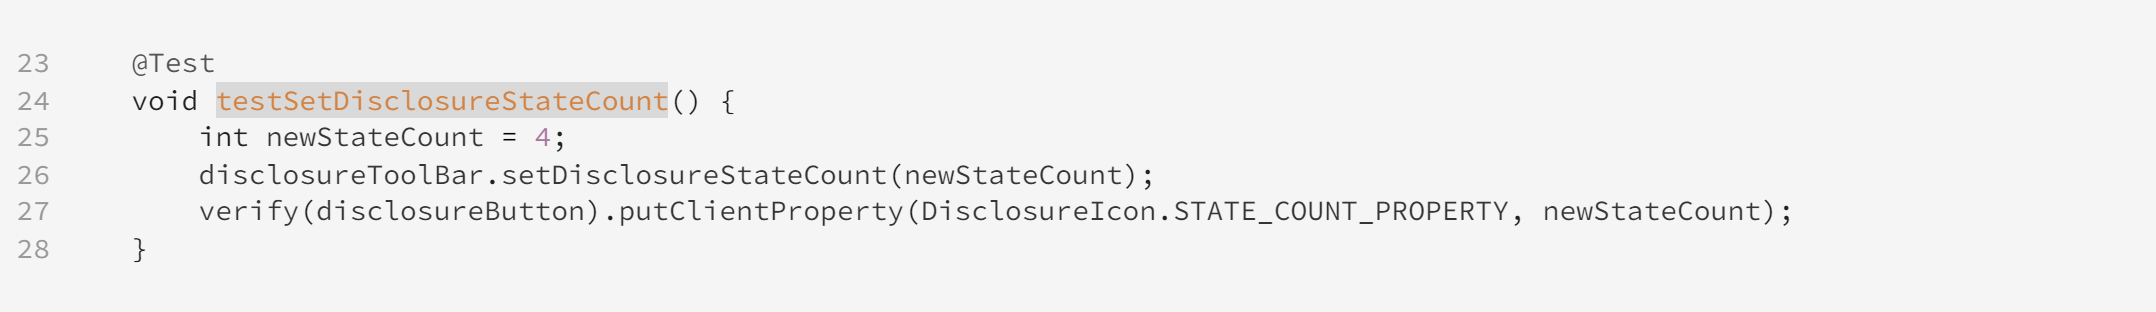
\includegraphics[width=\linewidth]{pic/Test testSetDisclosureStateCount.png}
    \caption{testtSetDisclosureStateCount Test}
    \label{fig:testSetDisclosureStateCount Test}
\end{figure}

\subsubsection{testGetDisclosureState}
This test is used to ensure that the getDisclosureState method correctly gets the current state of the disclosure button.
The test mocks the return value of the state and checks if the method returns this mocked value.

\begin{figure}[H]
    \centering
    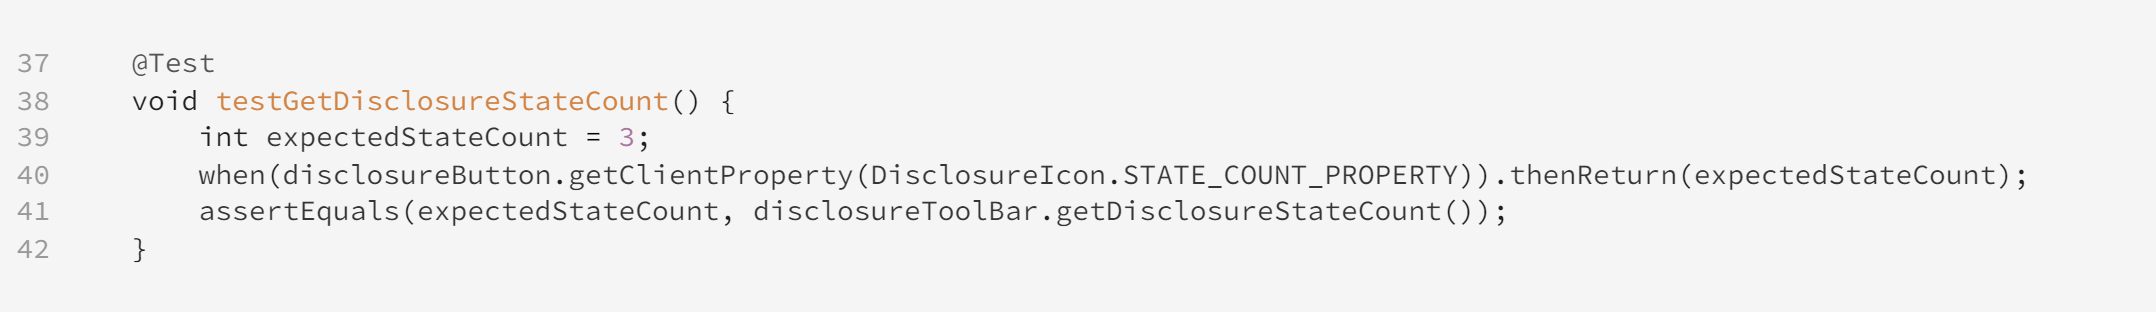
\includegraphics[width=\linewidth]{pic/Test testGetDisclosureStateCount.png}
    \caption{testGetDisclosureStateCount Test}
    \label{fig:testGetDisclosureStateCount Test}
\end{figure}

\subsubsection{testGetDisclosureStateCount}
This tests the getDisclosureStateCount method to check if it does return the correct count of disclosure states.
The test does this by setting an expected state count, mocking the retrieval, and checking if the returned count matches the expected value.

\begin{figure}[H]
    \centering
    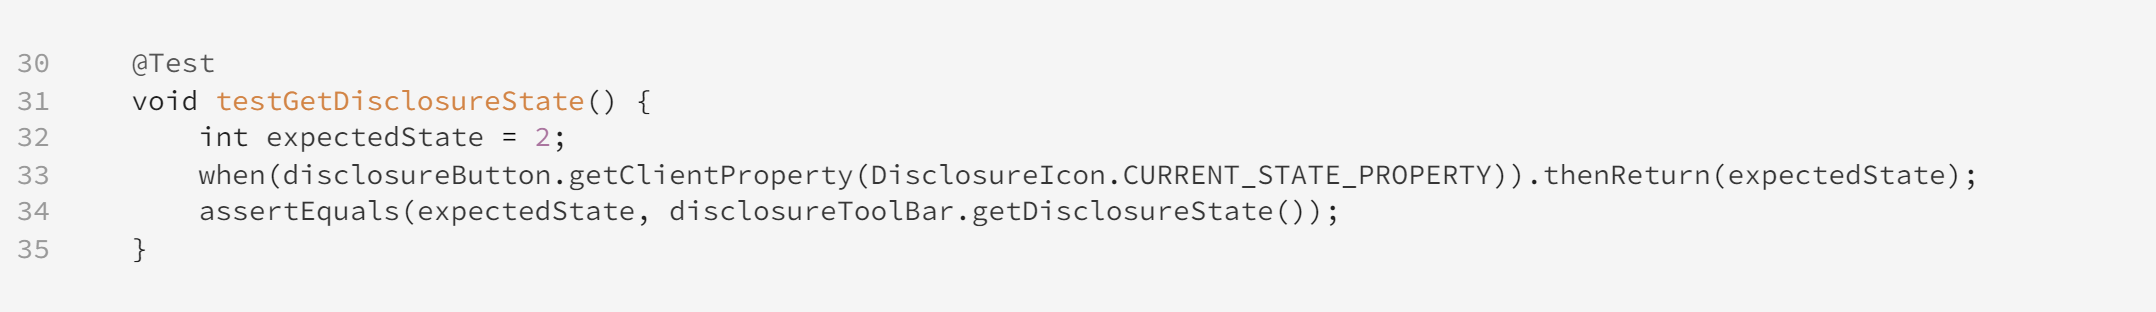
\includegraphics[width=\linewidth]{pic/Test testGetDisclosureState.png}
    \caption{testGetDisclosureState Test}
    \label{fig:testGetDisclosureState Test}
\end{figure}




\subsubsection{PaletteToolBarUI Tests}
The unit test for the \textit{PaletteToolBarUI} class, are unit tests were implemented to assure that when the tool palette is floating and trying to dock, functionalities are
working as inteded.
These tests are important when it comes to verifying the behavior of the toolbar.

\subsubsection{testSetFloatingTrue}
This test checks the setFloating method when the toolbar is set to float.
It cheks that when the floating state is set to true, the toolbars isFloating method shows this change of the state.

\begin{figure}[H]
    \centering
    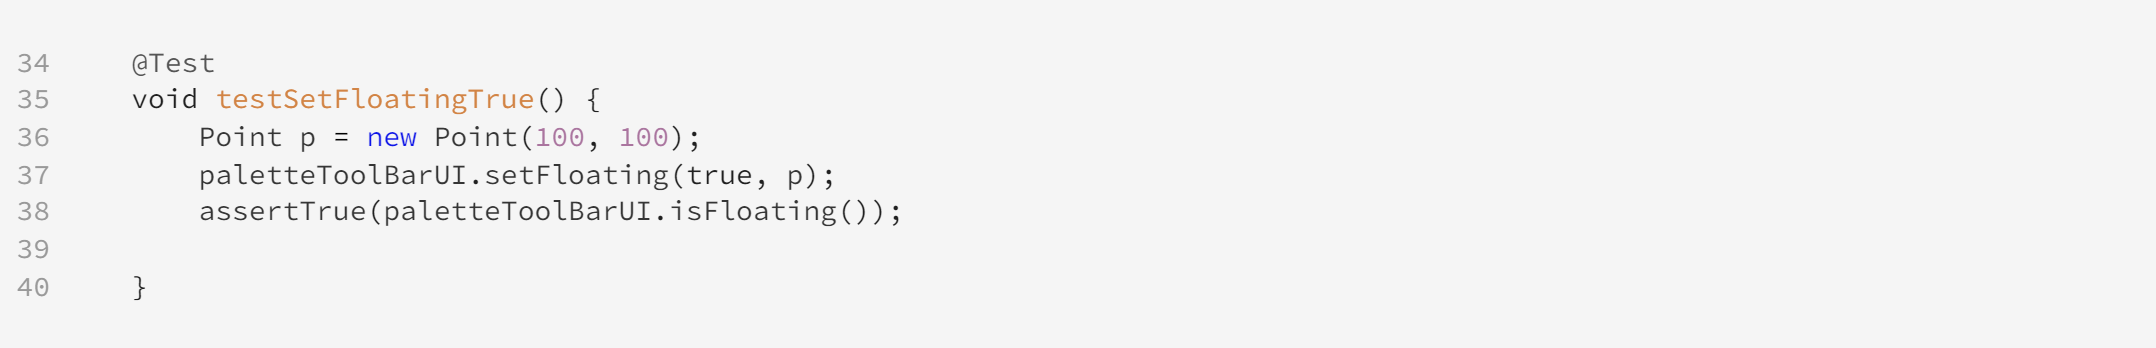
\includegraphics[width=\linewidth]{pic/Test testSetFloatingTrue.png}
    \caption{testSetFloatingTrue Test}
    \label{fig:testSetFloatingTrue Test}
\end{figure}




\subsubsection{testSetFloatingFalse}
This test checks the scenario where the toolbar is set to not be floating.
It well ensure that setting the floating state to false is correctly shown in the toolbars state.

\begin{figure}[H]
    \centering
    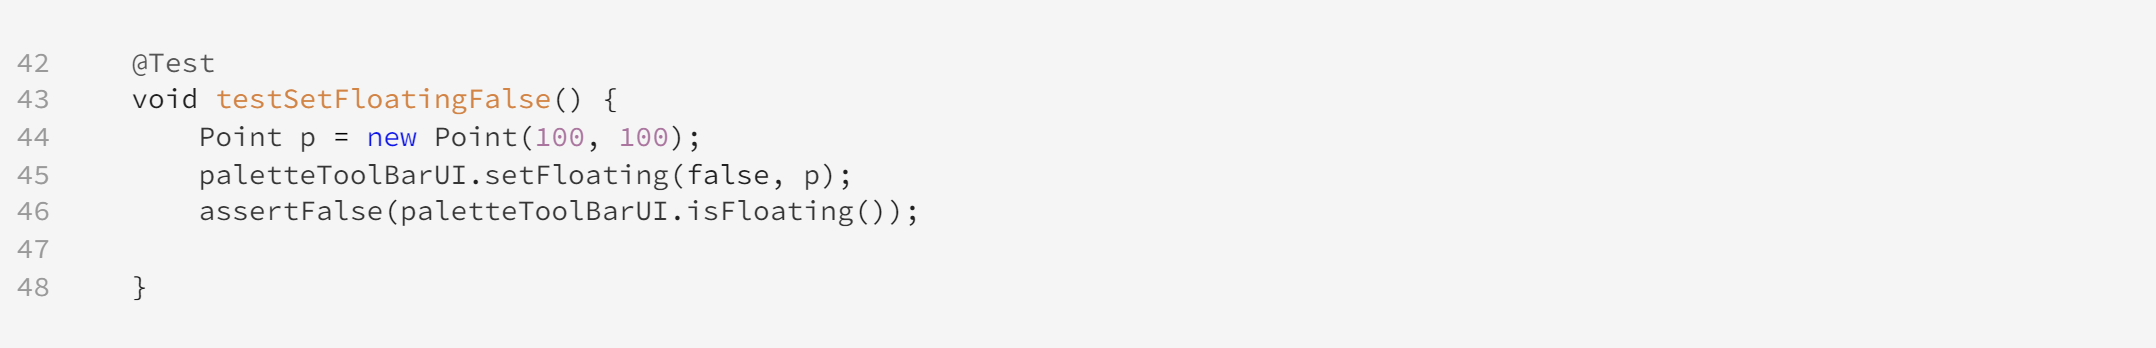
\includegraphics[width=\linewidth]{pic/Test testSetFloatingFalse.png}
    \caption{testSetFloatingFalse Test}
    \label{fig:testSetFloatingFalse Test}
\end{figure}




\subsubsection{testSetFloatingLocation}
This test checks the setFloatingLocation method.
It ckechs that the method correctly updates the floating coordinates of the toolbar.

\begin{figure}[H]
    \centering
    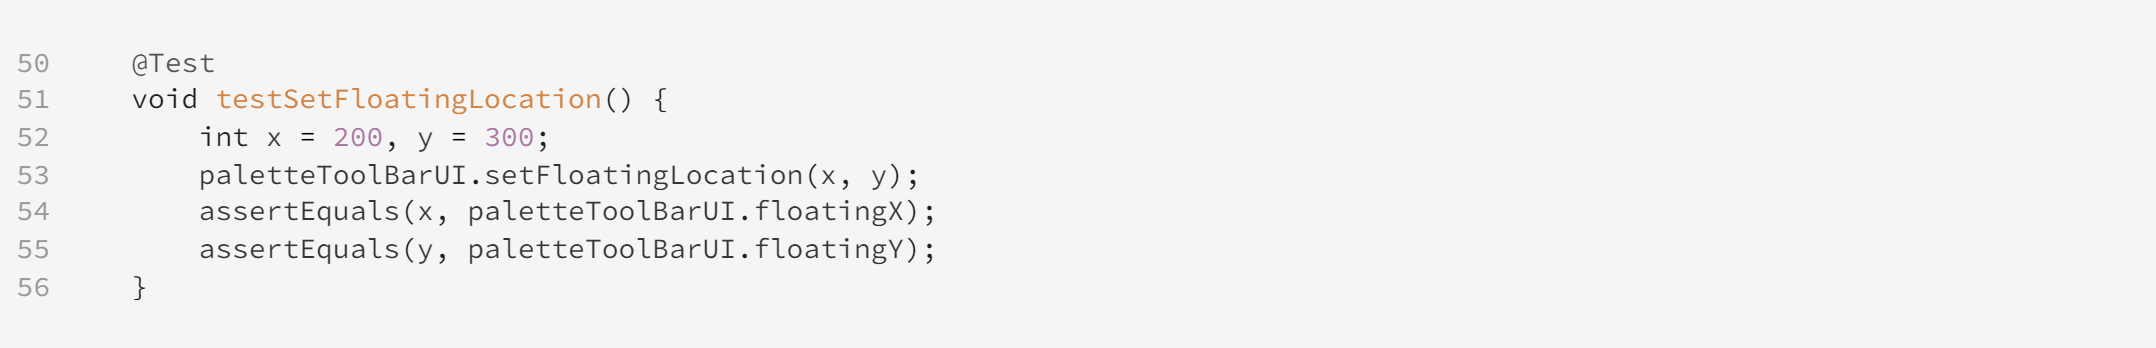
\includegraphics[width=\linewidth]{pic/Test testSetFloatingLocation.png}
    \caption{testSetFloatingLocation Test}
    \label{fig:testSetFloatingLocation Test}
\end{figure}




\subsubsection{testFloatAt}
This test checks the floatAt method, which is responsible for updating the toolbars position when dragged.
The test simulates the dragging action and checks the outcome is correct.

\begin{figure}[H]
    \centering
    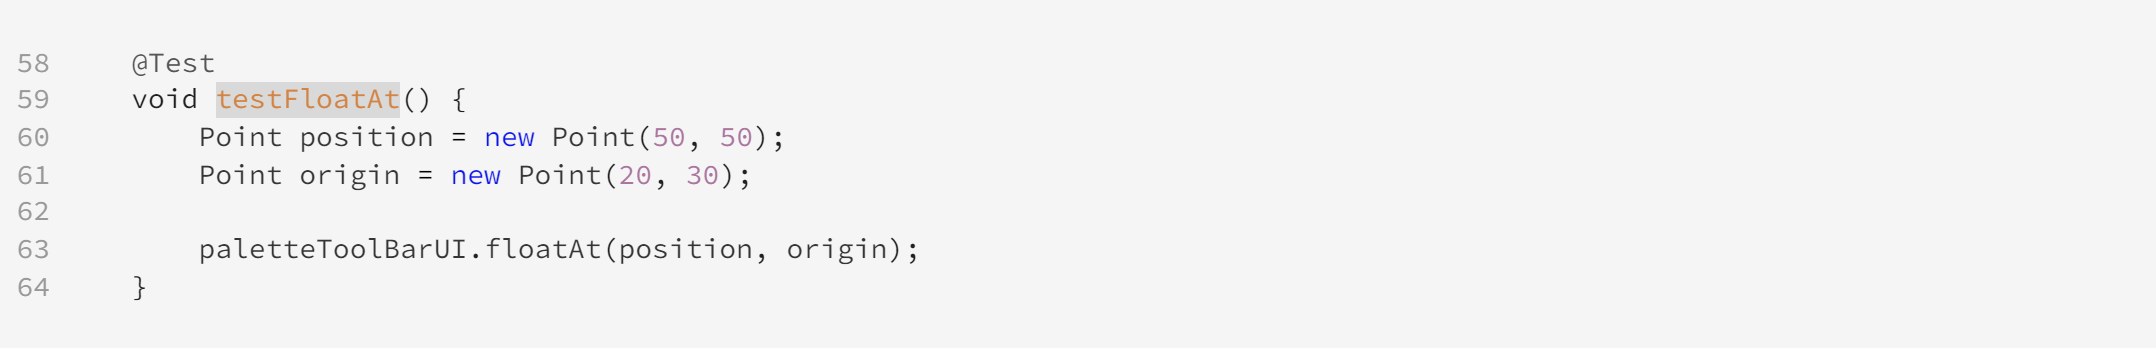
\includegraphics[width=\linewidth]{pic/Test testFloatAt.png}
    \caption{testFloatAt Test}
    \label{fig:testFloatAt Test}
\end{figure}


\subsection{Behavior-Driven Testing (BDD)}
The BDD focuses on application behavior from the user perspective. I used JGiven to make the BDDs automatically generated.

\subsubsection{ToolPaletteTestDisplay Scenario}
This scenario, \textit{scenario\_The\_user\_wants\_to\_hide\_a\_palette\_on\_the\_tool\_bar}, tries to mimic when a user wants to hide a toolbar palette from the toolbar itself.
The scenario code is build by 4 files \textit{GivenToolPaletteDisplay, ThenOutcomeDisplay, WhenUserInteractsDisplay} and \textit{ToolPaletteTestDisplay}.

The \textit{ToolPaletteTestDisplay} file is the main file that runs the scenario, and the other files are extended by it. below is the output when the scenario is run.


\begin{figure}[H]
    \centering
    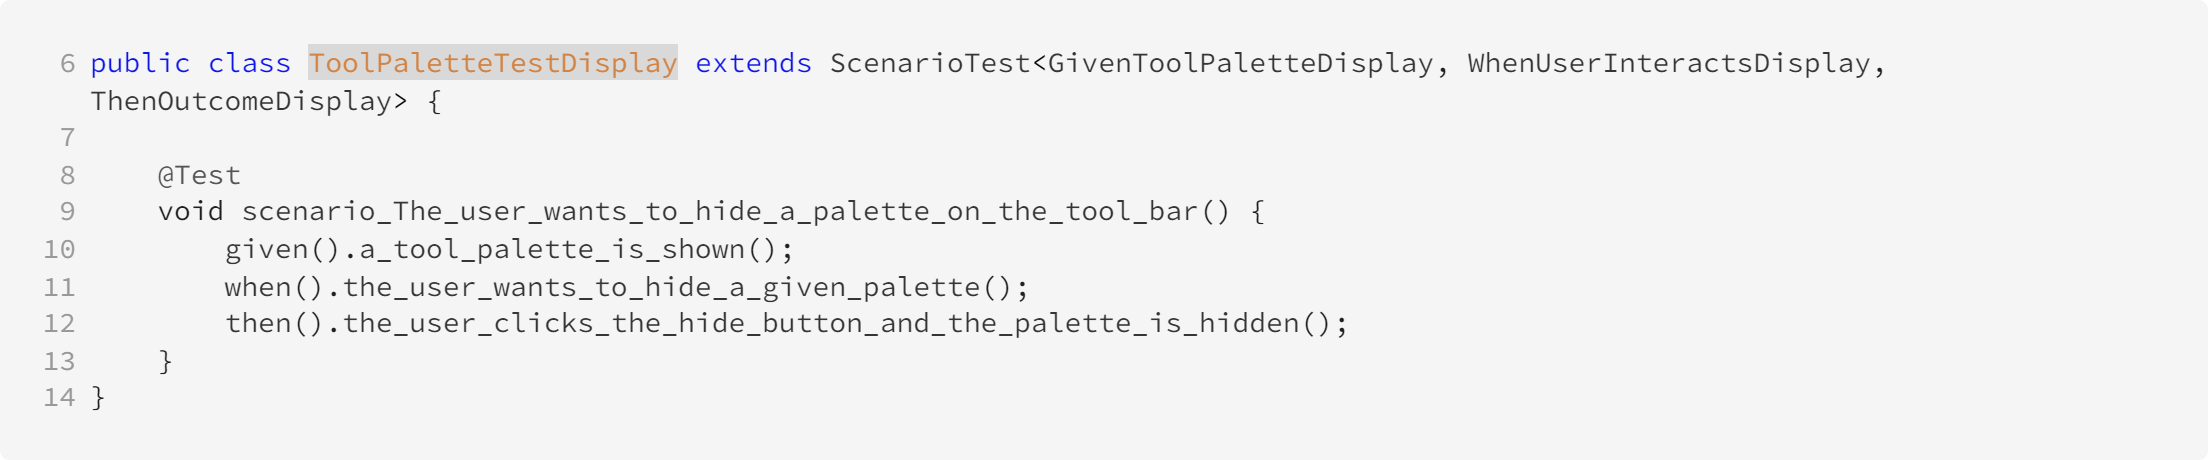
\includegraphics[width=\linewidth]{pic/BDD ToolPaletteTestDisplay.png}
    \caption{BDD ToolPaletteTestDisplay}
    \label{fig:BDD ToolPaletteTestDisplay}
\end{figure}



\begin{figure}[H]
    \centering
    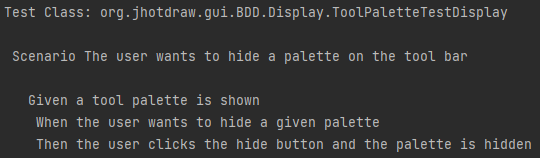
\includegraphics[width=\linewidth]{pic/BDD ToolPaletteTestDisplay output.png}
    \caption{BDD ToolPaletteTestDisplay output}
    \label{fig:BDD ToolPaletteTestDisplay output}
\end{figure}



\subsubsection{ToolPaletteTestDragAndDrop Scenario}
The \textit{ToolPaletteTestDragAndDrop} scenario minic an user interaction with drag-and-drop functionality in the toolbar.
The scenario code is build by 4 files \textit{GivenToolPaletteDragAndDrop, ThenOutcomeDragAndDrop, WhenUserInteractsDragAndDrop} and \textit{ToolPaletteTestDragAndDrop}.

The \textit{ToolPaletteTestDragAndDrop} file is the main file that runs the scenario, and the other files are extended by it. below is the output when the scenario is run.

\begin{figure}[H]
    \centering
    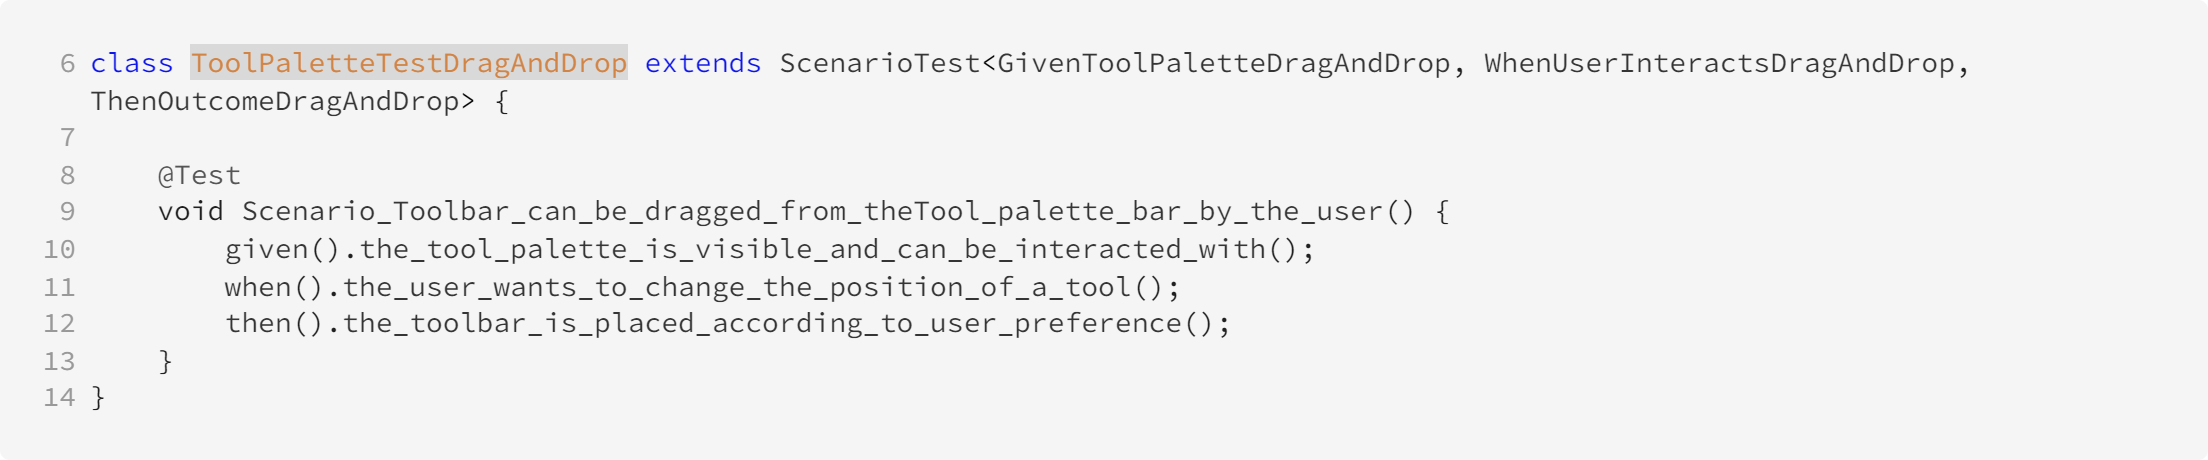
\includegraphics[width=\linewidth]{pic/BDD ToolPaletteTestDragAndDrop.png}
    \caption{BDD ToolPaletteTestDragAndDrop}
    \label{fig:BDD ToolPaletteTestDragAndDrop}
\end{figure}



\begin{figure}[H]
    \centering
    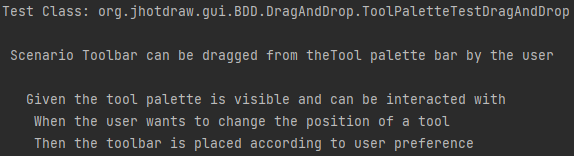
\includegraphics[width=\linewidth]{pic/BDD ToolPaletteTestDragAndDrop output.png}
    \caption{BDD ToolPaletteTestDragAndDrop output}
    \label{fig:BDD ToolPaletteTestDragAndDrop output}
\end{figure}